\documentclass[tikz,margin=3.14mm]{standalone}

\usepackage{tikz}
\usetikzlibrary{arrows}

\begin{document}
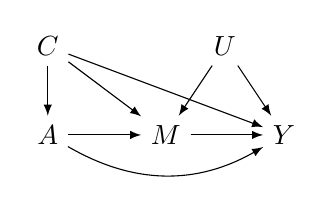
\begin{tikzpicture}[scale=1.5]

\node (A) at (0,0) {$A$};
\node (M) at (1,0) {$M$};
\node (Y) at (2,0) {$Y$};
\node (U) at (1.5,.75) {$U$};
\node (C) at (0,.75) {$C$};

\path [-latex] (A) edge [bend right] (Y);
\path [-latex] (A) edge (M);
\path [-latex] (M) edge (Y);
\path [-latex] (C) edge (A);
\path [-latex] (C) edge (M);
\path [-latex] (C) edge (Y);
\path [-latex] (U) edge (M);
\path [-latex] (U) edge (Y);
\end{tikzpicture}
\end{document}